\documentclass[10pt]{article}
\usepackage{itcep, stmaryrd, tikz, pgflibraryplotmarks, multicol, pgfplots}
\usepackage[margin=1in, nohead, pdftex]{geometry}

\topmargin -0.2in
\pagestyle{empty}
\singlespacing
\let\oldhat\hat
\renewcommand{\vec}[1]{\mathbf{#1}}
\renewcommand{\hat}[1]{\oldhat{\mathbf{#1}}}

\definecolor{light-gray}{gray}{0.95}
\newcommand{\code}[1]{\colorbox{light-gray}{\texttt{#1}}}

\newcommand{\headerclass}{Machine Learning Camp}
\newcommand{\headersection}{Day 2: Introduction to Classification}
\newcommand{\headertitle}{Iris Flower Dataset}

\def\C{\mathbb{C}}
\def\R{\mathbb{R}}
\parindent 0ex
\begin{document}
%==================================================================================================================================================
\headerclass\xspace \hspace{\stretch{1}} \headersection\\
\begin{center}{ \large \textbf{\headertitle} }\end{center}
%==================================================================================================================================================

To practice using the $k$-nearest neighbor algorithm in python, we'll be using a very famous dataset, the \emph{Iris flower data set} from statistician and biologist Ronald Fisher in 1936. This dataset consists of measurements taken from 150 iris flowers from three different iris species, Iris setosa, Iris virginica, and Iris versicolor. Four features were measured for each flower sample: sepal length, sepal width, petal length, and petal width.\\

\begin{minipage}{.5\textwidth}
\begin{center}
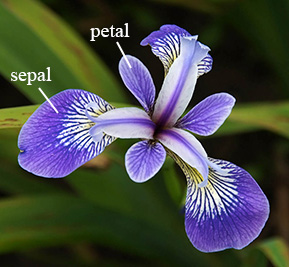
\includegraphics[height = 1.5in]{iris_with_labels}
\end{center}
\end{minipage}
\begin{minipage}{.5\textwidth}
The \emph{petals} are the colorful leaves of a flower, which surround the reproductive parts of the flower.\\

The \emph{sepals} are outside of the petals, and they protect the flower while it's in bud. When the flower blooms, the sepals support the petals. In most flowers, the sepals are green, but for these irises, the sepals are purple.
\end{minipage}\\

When Fisher first introduced the iris data set, he showed how a machine learning method called \emph{linear discriminant analysis} can be used for classification of these iris species. Since then, the Iris dataset has become one of the most commonly used datasets for practicing, testing, and demonstrating machine learning classification algorithms. As you continue to study machine learning, you're likely to come across the iris dataset again and again!

\vfill

\begin{center}{ \large \textbf{Breast Cancer Dataset} }\end{center}

Another famous dataset is the Wisconsin breast cancer dataset. This dataset consists of measurements taken from an image of a breast mass, and these measurements describe the shape of the cell nuclei visible in the image. Each sample is classified as malignant or benign, telling us if it is a cancerous cell. The dataset contains measurements from 357 benign samples, and 212 malignant samples. \\

\begin{minipage}{.5\textwidth}
\begin{center}
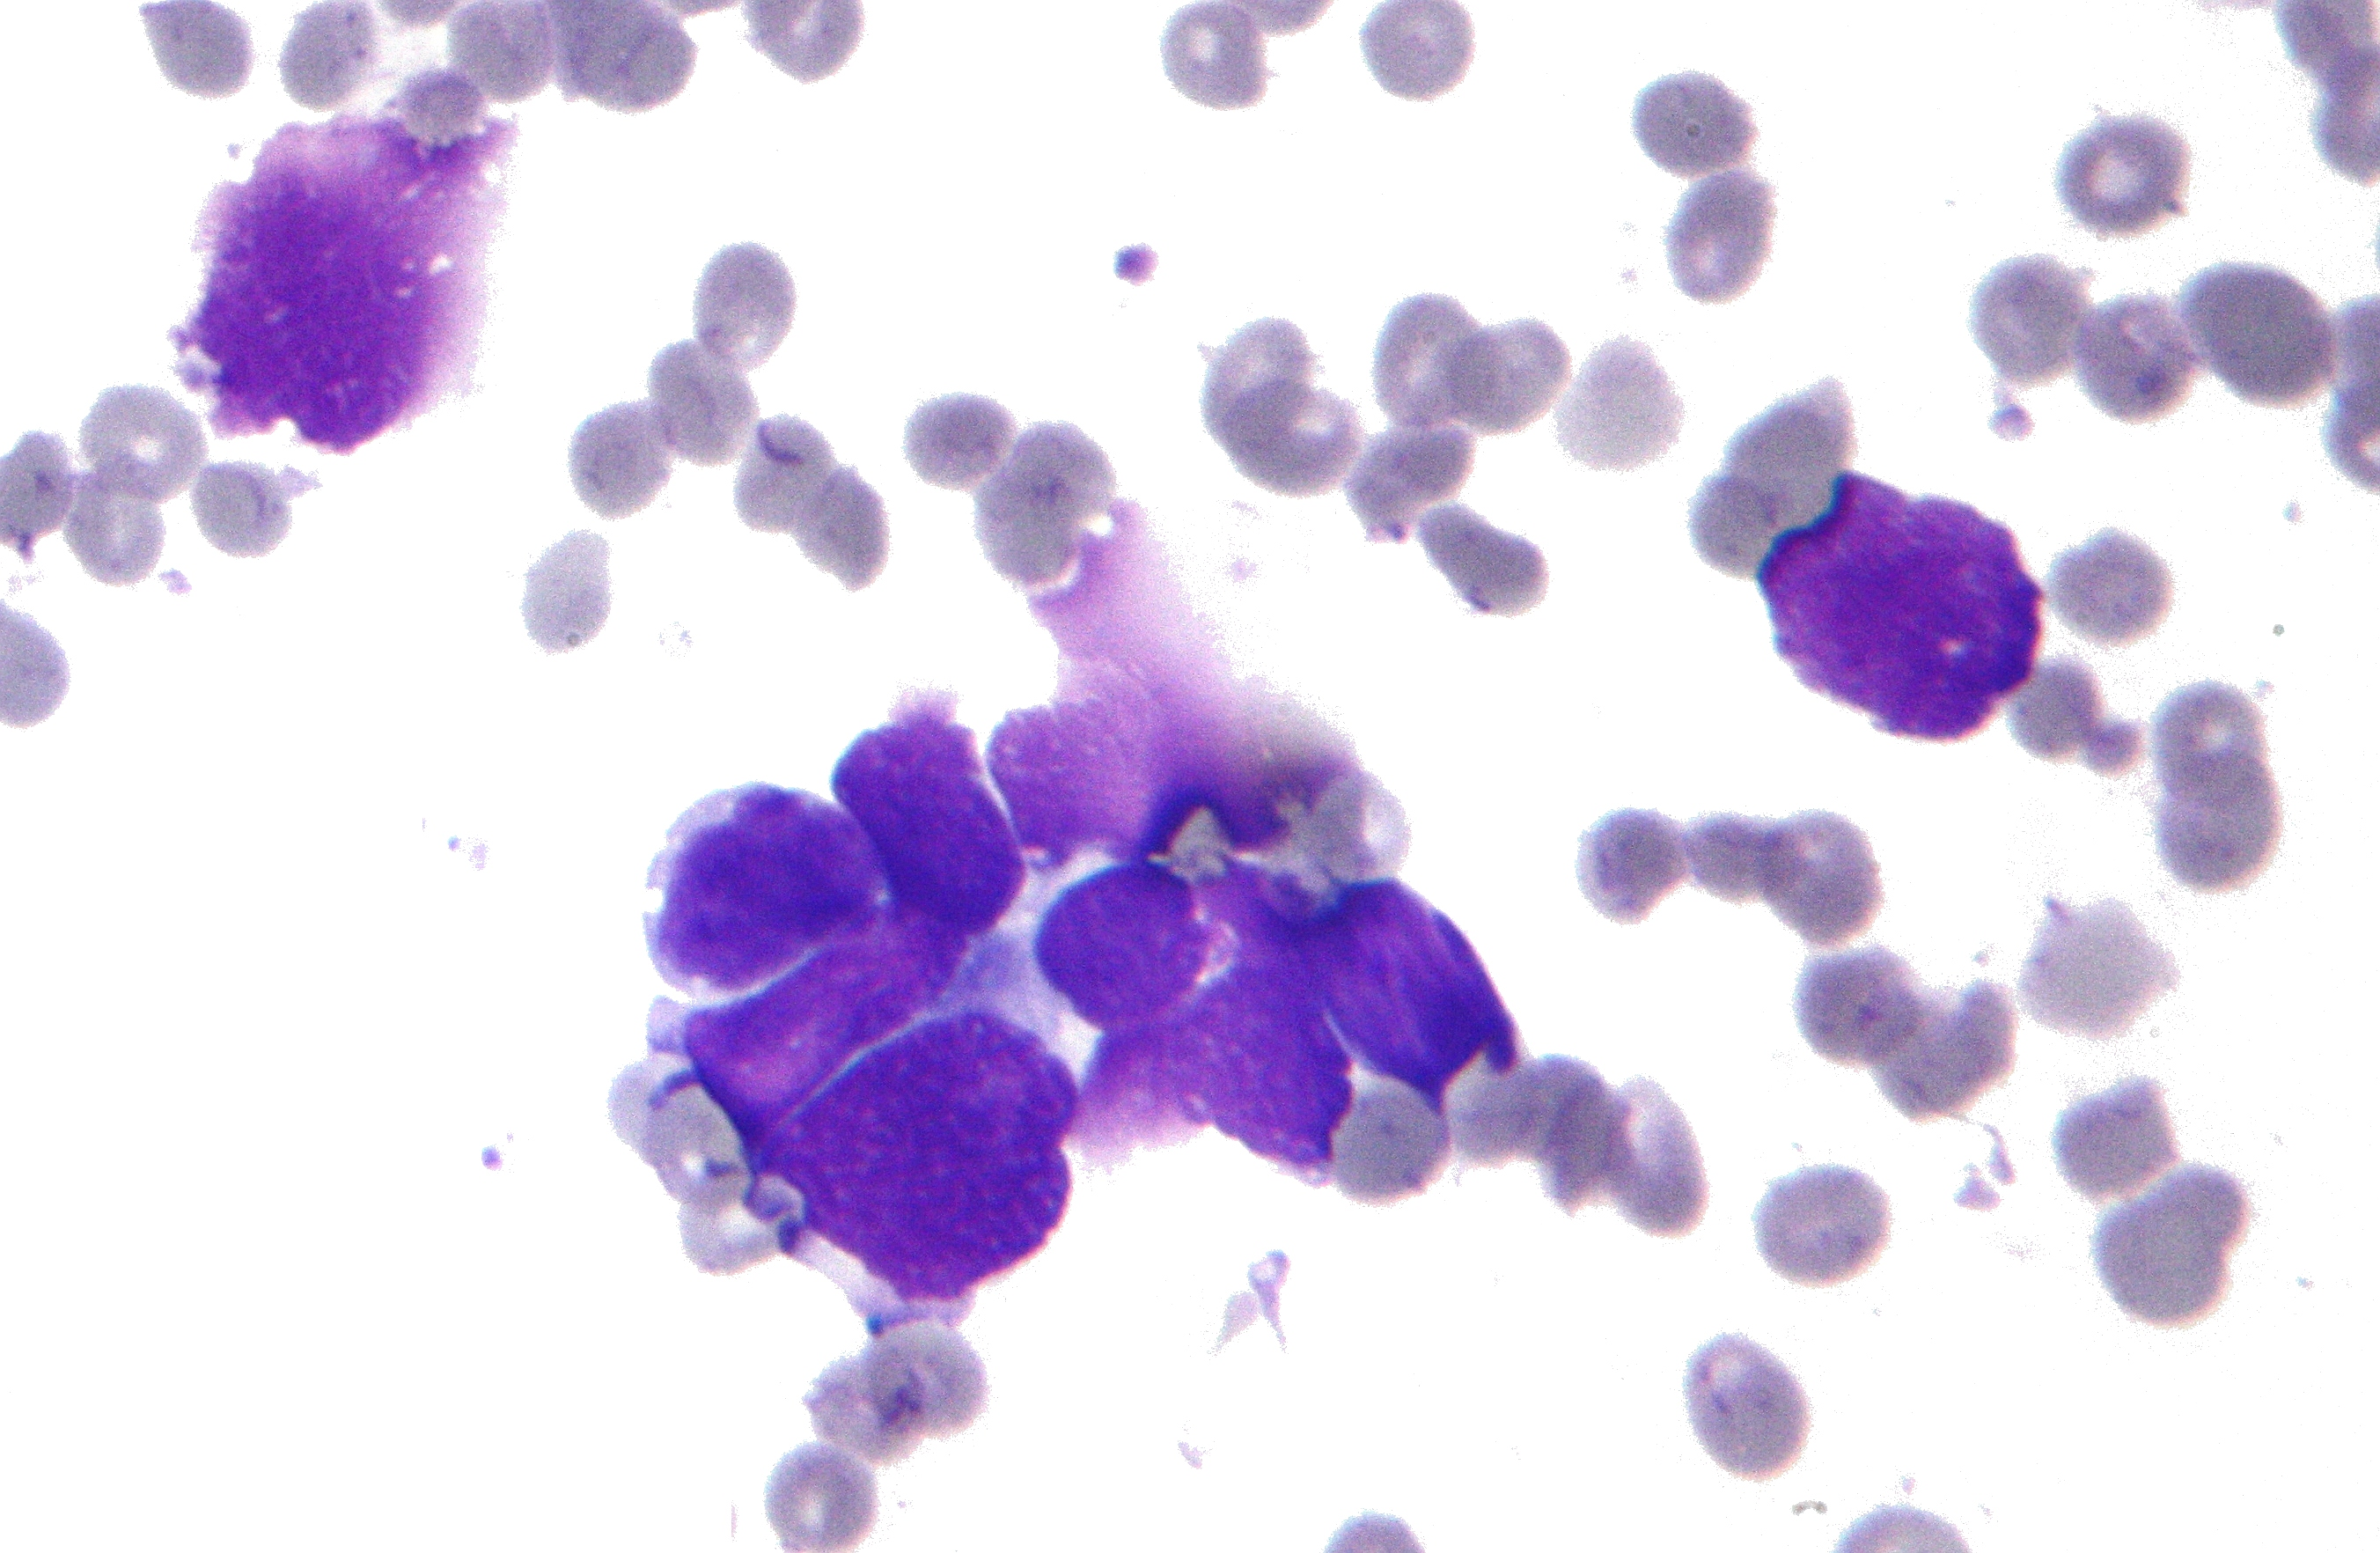
\includegraphics[height = 1.5in]{dataset-original}
\end{center}
\end{minipage}
\begin{minipage}{.5\textwidth}
The following measurements were taken for each nucleus in each image: radius, texture, perimeter, area, smoothness, compactness, concavity, number of concave points, symmetry, and fractal dimension.\\

For each image, the mean, standard error, and average of the three largest values were computed over all nuclei in the image. These measurements are the features in the dataset.
\end{minipage}\\

The goal of studying this dataset is to answer the question: can we predict if a sample is cancerous or not, based on measurements of the shape of the cells? This would be useful as an initial screening procedure; if the cells appear to be cancerous, further tests could then confirm this preliminary diagnosis.
\vfill


\end{document}
